%============================ MAIN DOCU =================================
% define document class
\PassOptionsToPackage{table}{xcolor}
\documentclass[
   10.5pt,
   invert-title=true,
   titlepage=false,
   titleimage-ratio=13,
   class=article
]{bfhpub}				% KOMA-script report
%---------------------------------------------------------------------------
% Documents paths
%---------------------------------------------------------------------------
\makeatletter
\def\input@path{{content/}}
%or: \def\input@path{{/path/to/folder/}{/path/to/other/folder/}}
\makeatother
%-----------------  Set default font family  -------------------------------
\renewcommand{\familydefault}{\sfdefault}
%-----------------  Base packages     --------------------------------------
% Include Packages
\usepackage[babel, german=quotes]{csquotes}
%---------------------------------------------------------------------------
\usepackage{blindtext}  %% For placeholder text only
%---------------------------------------------------------------------------
\usepackage{geometry}
\geometry{
   a4paper, % Papierformat
   top=3cm, bottom=4cm, % Rand oben/unten
   outer=2.5cm, inner=3cm % aussen/inne
}
%---------------------------------------------------------------------------
%\usepackage[
%  backend=biber,
%  style=alphabetic,
%  sorting=ynt
%]{biblatex}
%\addbibresource{sample.bib} %% Name of bibliography file
%---------------------------------------------------------------------------
\usepackage{multicol}
%---------------------------------------------------------------------------
% Hyperref Package (Create links in a pdf)
%---------------------------------------------------------------------------
\usepackage[
   hidelinks
  ,colorlinks
  ,linkcolor=.
  ,filecolor=.BFH-MediumGreen
  ,urlcolor=BFH-MediumBlue
  ,citecolor=.
  ,plainpages=false
  ,pdfpagelabels
  ,pdfusetitle
  ,hypertexnames = {true},	% no failures "same page(i)"
]{hyperref}
%---------------------------------------------------------------------------

\usepackage{xcolor}
\usepackage{listings}

\definecolor{mGreen}{rgb}{0,0.6,0}
\definecolor{mGray}{rgb}{0.5,0.5,0.5}
\definecolor{mPurple}{rgb}{0.58,0,0.82}
\definecolor{backgroundColour}{rgb}{0.95,0.95,0.92}
\usepackage{color} %red, green, blue, yellow, cyan, magenta, black, white
\definecolor{mygreen}{RGB}{28,172,0} % color values Red, Green, Blue
\definecolor{mylilas}{RGB}{170,55,241}

\lstset{language=Matlab,%
	%basicstyle=\color{red},
	breaklines=true,%
	morekeywords={matlab2tikz},
	keywordstyle=\color{blue},%
	morekeywords=[2]{1}, keywordstyle=[2]{\color{black}},
	identifierstyle=\color{black},%
	stringstyle=\color{mylilas},
	commentstyle=\color{mygreen},%
	showstringspaces=false,%without this there will be a symbol in the places where there is a space
	numbers=left,%
	numberstyle={\tiny \color{black}},% size of the numbers
	numbersep=9pt, % this defines how far the numbers are from the text
	emph=[1]{for,end,break},emphstyle=[1]\color{red}, %some words to emphasise
	%emph=[2]{word1,word2}, emphstyle=[2]{style},    
}

\usepackage{bfhterminal}
\usepackage{bfhboxes}
\usepackage{hyperref}

\newcommand*{\code}[1]{\enquote{\texttt{#1}}}  %% The "code" macro definition

\graphicspath{ {./pics/} }

\colorlet{BFH-Title}{white}

\begin{document}
\setlength{\parskip}{0pt}
\setlength{\parindent}{0pt}
  %----------------  BFH tile page   -----------------------------------------
  \title{Titanic-Matlab}
  \subtitle{Using Classification Learner in Matlab}
  \author{Till Moser and Sebastian von Allmen}
  \subject{BZG1308ab}
%  \publishers{publishers}
  \institution{Bern University of Applied Sciences}
  \department{Technik und Informatik}
  \institute{Mikro- und Medizintechnik}
  \version{1.0}
  %The starred variant will automatically scale and clip the image. the non-starred one will allow you to set the size yourself
%  \titlegraphic*{\includegraphics{example-image}}
  
  \maketitle
  %------------ TABLEOFCONTENTS ---------------
%  \tableofcontents

\section*{Abstract}
%\includegraphics[width=6cm]{flower}
\textbf{In this Documentation we will give you a brief overview of how Machine Learning works and how you can use it in Matlab. More specifically we will talk about the classification learner in Matlab. This will give you a powerfull tool for Data analysis and you can use the gained knowledge with the Regression Learner.\newline
To do this we used a online Machine Learning Competition. \href{https://www.kaggle.com/c/titanic}{Kaggle-Titanic}. It is a very popular Competition for people who are trying to get into Data Science. Therefore there are a lot of online guides for it. We combined the knowledge we gained from them for this report. The goal of the competition is to guess who survived the sinking of the Titanic and who did not. To help you guess you get a train.csv file with information about the people on board. 
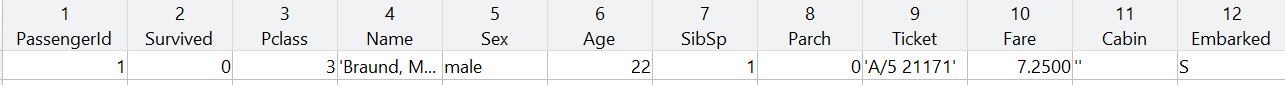
\includegraphics[width=155mm\\]{data} 
\newline
You use this data to train your Model. After developing your Model the true test comes. You run it using the test.csv file. This contains the same information but not whether or not the Passenger survived. To guess this you use your Model. How accurate this guess is, shows how good your model was developed}

\section*{Introduction}
You can group the Machine Learning the following way. 
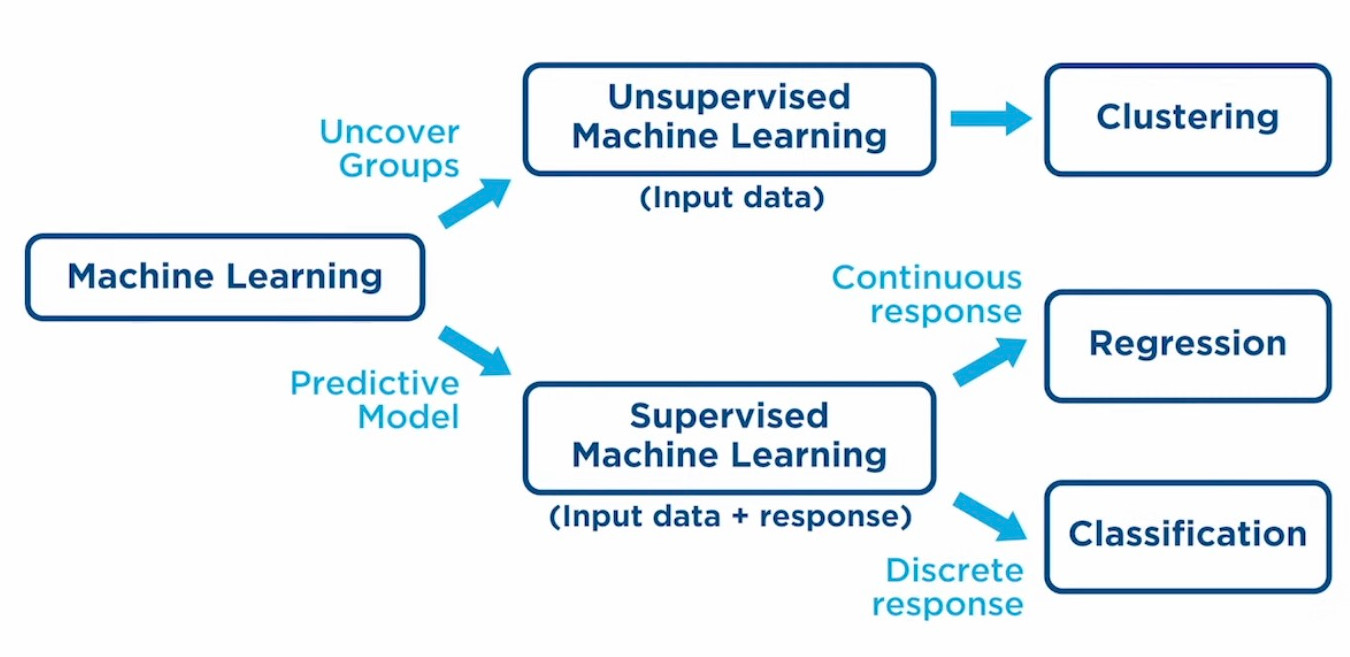
\includegraphics[width=80mm\\]{overview}
\newline
We will focus on the Classification of Supervised Learning. This means the output comes out to be in one class. I.e. Survived or did not Survive. It could also be Apple, Banana or Orange. A Regression problem would f.e. be how much taxes you have to pay. I.e. 698.5 chf or 1045.7 chf. To do Supervised Machine Learning in Matlab we used the Classification Learner. Before diving in to that, we want to explain how the general Process of Machine Learning works. This graphic show the process.
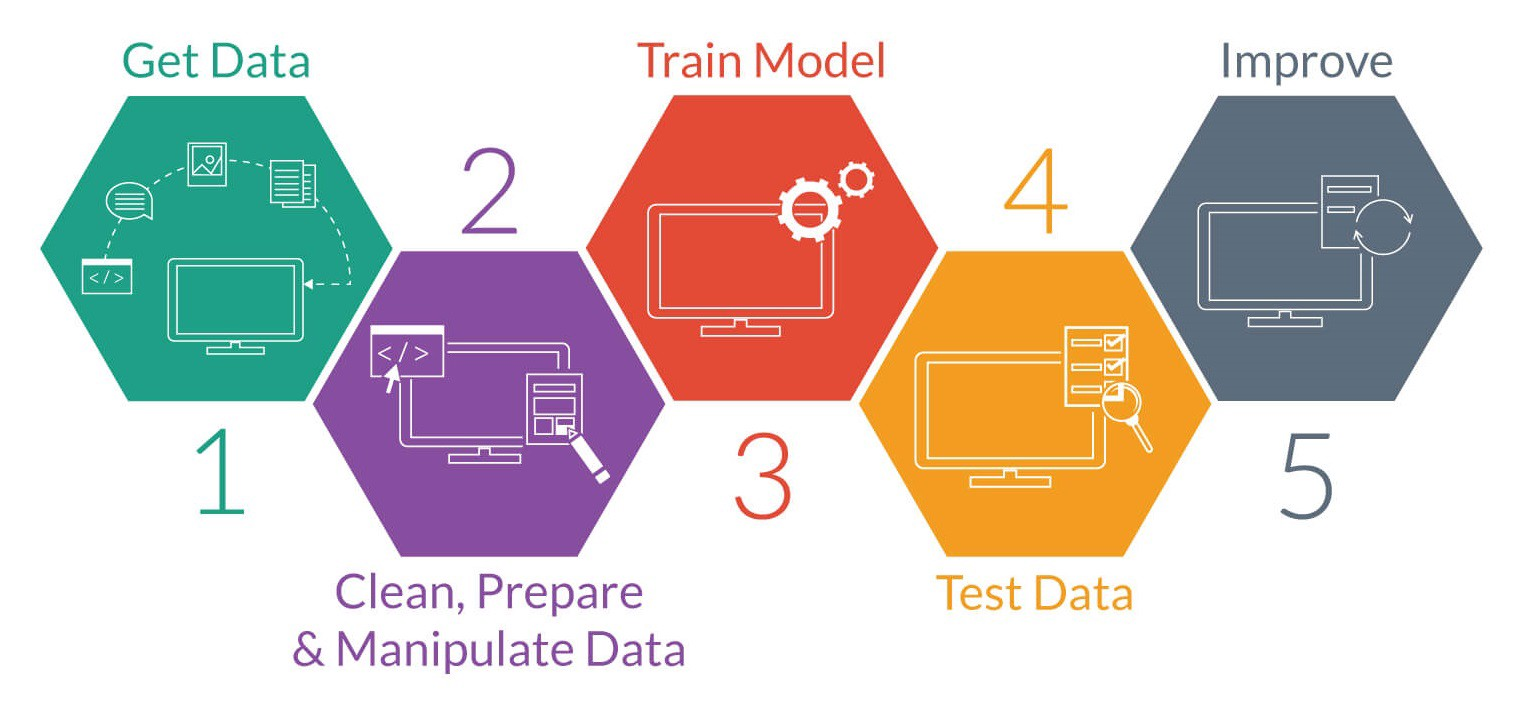
\includegraphics[width=70mm\\]{process}
\subsection*{Get Data}
First you have to get your data. This will most of the time be the easy part. In our case we just have to read in the data from the .csv File.
%%Villech gits da öppis Matlab spezifisches has bis iz ni gfunde
\begin{lstlisting}[language=Matlab]
Test = readtable('test.csv','Format','%f%f%q%C%f%f%f%q%f%q%C');
\end{lstlisting}

\subsection*{Clean Data}
It is highly likely that you will have some blank spots in your data. To fill them is your responsibility. You will also likely have some Data that is non relevant to solving your Problem. To remove them is also your job. In code this would look something like this.

\begin{lstlisting}[language=Matlab]
avgAge = nanmean(Train.Age)          
Train.Age(isnan(Train.Age)) = avgAge;  
Test.Age(isnan(Test.Age)) = avgAge;    
\end{lstlisting}

\subsection*{Train Model}
We train the Model using the Classification Learner from the Matlab Toolbox. You can read more about it in its own section. 
 
\subsection*{Test Data}
To test the Data we have two options. We can test run it against the training Data. This will give us a good estimate of how good the model performs. It should be pretty good since it is the same data we used to Train the Model. If we want to do a real test, we should run it against the test Data. We do not know the outcome for this data. To check how good we were we can upload this data to Kaggle. It will tell us our success rate. 

\subsection*{Improve}
Now we get ti the interesting Part. To improve our Model we have two options. The first option is we find a better Model and train it more. The other option is to clean prepare and Manipulate the Data in a smarter Way by including intelligent features and removing unimportant Data.


\section*{Methology}
To create your own Machine Learning Model you first have to learn the basics. We used this tutorial for that \href{https://blogs.mathworks.com/loren/2015/06/18/getting-started-with-kaggle-data-science-competitions/}{Matlab-Tutorial}.
This will teach you the basics and you will be able to develop your own models after completing it.

\subsection*{Classification Learner}

\subsection*{Sebasmodell}
In my Model i decided to use the boosted Tree Algorithm. The boosted Tree Algorithm is basically just a lot of decision Trees combined. The Algorithm combines a lot of weak learners in series to create a strong learner model. It works differently than a random Forest Model.
I tried to improve the performance of the Model by including some clever feature Datatypes and by improving how i filled out blank spaces.

\subsection*{Tillsmodel}

\section*{Results}
In the end we developed two individuell Models that worked better than primitive guesses. We are really happy with that. The primitive guess would be to say every woman survived and every man died.

\begin{center}
	\begin{tabular}{ c c }
		Method & Acuraccy in [\%] \\
		primitve & cell2 \\ 
		sebasmodel & 77.2 \\
		tillmodel & cell8    
	\end{tabular}
\end{center}

\section*{Discussion}



  %------------ BIBLIOGRAPHY ---------------
%\printbibliography

\end{document}
